% vim: set tabstop=4 :
%**********************************************************
%\chapter{提案手法にあたる章}
%\chapter{格子分割を用いた進行方向計算の削減手法}
\chapter{格子分割による進行方向ベクトル計算の削減手法}
\label{sec:method}
%**********************************************************
SFMの運動方程式は,エージェントの位置が変わるたびに,
目的地までのベクトルを表す$e$や周囲のエージェントを避ける力$f_{ij}$,
障害物を避ける力$f_{iW}$の再計算が必要となる.
周囲のエージェントを避ける力$f_{ij}$の計算は,時間ステップごとにすべての
エージェントの位置が変化するため,解析中のみに計算が可能である.
一方,ベクトル$e$や障害物を避ける力$f_{iW}$は,エージェントの位置に
応じて決定し,壁や机などの障害物の座標が固定であることから,解析前に計算が可能である.

そこで,本論文では,格子状に分割した領域ごとにベクトル$e$と障害物を避ける力$f_{iW}$を
あらかじめ計算することで,解析中の進行方向の再計算を削減する.

\section{格子分割を用いた進行方向計算手法}
本手法は,解析領域を格子状に分割し,格子ごとに進行方向ベクトル$e$や
障害物を避ける力$f_{iW}$をあらかじめ計算する.
進行方向ベクトル$e$は,式\eqref{eq:sfm_siki1}に示すSFMの運動方程式から
$v_i^0(t)$が係数である.一方で,障害物から受ける力$f_{iW}$は,
式\eqref{eq:sfm_siki1}に示すように,式の第3項である.
このため,進行方向ベクトル$e$と障害物を避ける力$f_{iW}$は,
別々の配列に格納する必要がある.
\figref{fig:5_teian_flow1}に格子分割を用いた
進行方向ベクトル計算の削減手法のフローチャートを示す.
\figref{fig:5_teian_flow1}中の前処理は,提案手法に必要である格子ごとの進行方向や
壁を避ける力を算出する.
\figref{fig:5_teian_flow1}中の運動方程式を用いた計算は,
エージェントの進行方向を計算する処理であり,
エージェントの進行方向ベクトル$e$や
障害物を避ける力$f_{iW}$を前処理で算出した値を参照する.

\figtb{提案手法の解析全体のフローチャート}{}{4.5}{5_teian_flow1.eps}{5_teian_flow1}

%\subsection{格子分割を用いた進行方向ベクトル$e$の計算方法}
\subsection{格子ごとの進行方向ベクトル$e$の計算方法}
進行方向ベクトル$e$は,目的地に進むベクトルであり,エージェントの座標から
目的地の座標までのベクトルである.
このため,ベクトル$e$は解析領域を格子状に分割した領域ごとの中心座標から
目的地の座標までのベクトルを計算することで,解析前に計算が可能となる.
\figref{fig:grid_ex1}に格子分割した進行方向の例を示す.
%
\figtb{提案する格子分割の例}{}{9}{ex1.eps}{grid_ex1}
%
\figref{fig:grid_ex1}中の○はエージェントであり,エージェントA,Bが1つの目的地に向かう
様子である.
図中のエージェントBは,エージェントAの位置に移動したとき,エージェントAと同じ進行方向に
なる.
このため,解析領域を分割し,格子ごとに進行方向を算出することで,解析中の
進行方向の再計算が削減できる.
目的地と障害物が含まれる格子は,エージェントが正しく目的地に進むようにするために,
0ベクトルを格納する.
0ベクトルが格納された格子中に存在するエージェントは,
改めて個別に進行方向ベクトル$e$を計算する.
格子ごとの進行方向は,格子の中心座標から目的地までのベクトル$e$を求め,配列に格納する.
目的地の他に経由地が複数存在する場合,進行方向は,経由地ごとに異なるため,経由地ごとに違う配列に格納する必要がある.
\figref{fig:ex2}に経由地が複数存在する例を示す.
\figref{fig:ex2}中の右図は経由地の進行方向,左図は目的地の進行方向,青色の矢印は経由地に進む進行方向,
青矢印は目的地の進行方向,0は進行方向を個別計算するための0ベクトル,オレンジ色の四角は机などの障害物を示す(要工事:元となる画像がない).
\figref{fig:ex2}のように,経由地と目的地の進行方向は,それぞれの座標が異なるため,ベクトル$e$も大きく異なることから,
それぞれ別の配列で保持する必要がある.
経由地ごとに別の配列に進行方向を格納するため,進行方向を格納する配列の要素数は
式\eqref{eq:route_youso_size}に進行方向を格納する要素数を示す.
%
\begin{eqnarray}
 \mbox{進行方向の格子の要素数[個]} = 
 \Big( \frac{\mbox{解析領域[m]}}{\mbox{格子サイズ[m]}} \Big) ^ 2 \times  2 \times \mbox{経由地数[個]}
 \label{eq:route_youso_size}
\end{eqnarray}
%
式\eqref{eq:route_youso_size}のように,進行方向を格納する配列は,
解析領域の大きさや格子サイズの小ささ,経由地数の大きさに応じて
要素数が増加する.
また,進行方向を格納する配列の前処理にかかる時間は,
配列の要素数に応じて格子ごとの進行方向計算回数が増加するため,
配列の大きさに応じて増加する.

\figtb{経由地がある場合の進行方向の例}{}{7}{ex2.eps}{ex2}

%\figtb{シミュレーション中の進行方向計算のフローチャート}{}{8.5}{5_e_flow.eps}{5_e_flow}

%\subsection{格子分割を用いた障害物を避ける力$F_{iW}$の計算方法}
\subsection{格子ごとの障害物を避ける力$F_{iW}$の計算方法}
障害物を避ける力$F_{iW}$は,エージェントの座標と障害物の座標に応じて変化する.
障害物は,机や壁などの固定された物であるため,座標が変化しない.
このため,障害物を避ける力$F_{iW}$は,解析領域を格子状に分割した領域ごとの
中心座標と障害物の座標から解析前にあらかじめ計算が可能となる.
\figref{fig:preparation_fiw}に格子分割した障害物を避ける力$F_{iW}$を示す.
\figref{fig:preparation_fiw}中の四角は解析領域を格子状に分割した格子,
黒点は格子の中心点,緑色の丸は格子の中心点からの影響範囲,オレンジ色の
丸は壁粒子,赤色の矢印は黒点の中心点が受ける障害物を避ける力$f_{iW}$である.
\figref{fig:preparation_fiw}の例は,黒点が存在する格子が受ける障害物を避ける力$f_{iW}$
を示しており,黒点の中心点から緑色の範囲に存在する壁粒子から力を受ける.
各格子は,\figref{fig:preparation_fiw}のように格子の中心点の座標を
用いて障害物を避ける力を計算する.
壁を避ける力$F_{iw}$を格納する配列は,
経由地が変わっても変化しないため,解析領域全体で一つとなる.
式\eqref{eq:fiw_youso_size}に障害物を避ける力$F_{iW}$を格納する配列の要素数を示す.
%
\begin{eqnarray}
 \mbox{障害物を避ける力を格納する格子の要素数[個]} =  \Big( \frac{\mbox{解析領域[m]}}{\mbox{格子サイズ[m]}} \Big) ^ 2 \times 2
 \label{eq:fiw_youso_size}
\end{eqnarray}
%
式\eqref{eq:fiw_youso_size}に示すように,障害物を避ける力を格納する配列の要素数は,
解析領域と格子サイズに応じて決まり,解析領域を格子サイズで割った値の二乗が配列の要素数となり,
障害物を避ける力$F_{iW}$がxとy方向に存在するため,要素を2倍した値が障害物を避ける力$F_{iW}$を
格納する配列の総要素数になる.
\figref{fig:5_teian_flow2}に格子分割を用いた進行方向の計算回数削減手法の前処理のフローチャート
を示す.
\figref{fig:5_teian_flow2}中の$F_{iW}$配列は障害物を避ける力$F_{iW}$を格納する配列,
進行方向配列は進行方向ベクトル$e$を格納する配列,
$F_{iW}$のxインデックスとyインデックスは$F_{iW}$配列に格納するためのインデックスであり,
すべての要素に値を格納するためのループである.
同様に,進行方向配列のxインデックスとyインデックスは進行方向ベクトル$e$を配列に格納するための
インデックスであり,すべての要素に値を格納するためのループである.
進行方向ベクトル$e$は,経由地ごとに異なるため,経由地数分のループが前処理に必要となる.


%障害物が含まれる格子と周辺の格子に0を入れることを書く.

\figtb{格子分割した障害物を避ける力$F_{iW}$の例}{}{8}{5_fiw_grid.eps}{preparation_fiw}

%\figtb{提案手法の前処理のフローチャート}{}{5}{5_teian_flow2.eps}{5_teian_flow2}

\begin{figure}[p]
 \begin{center}
  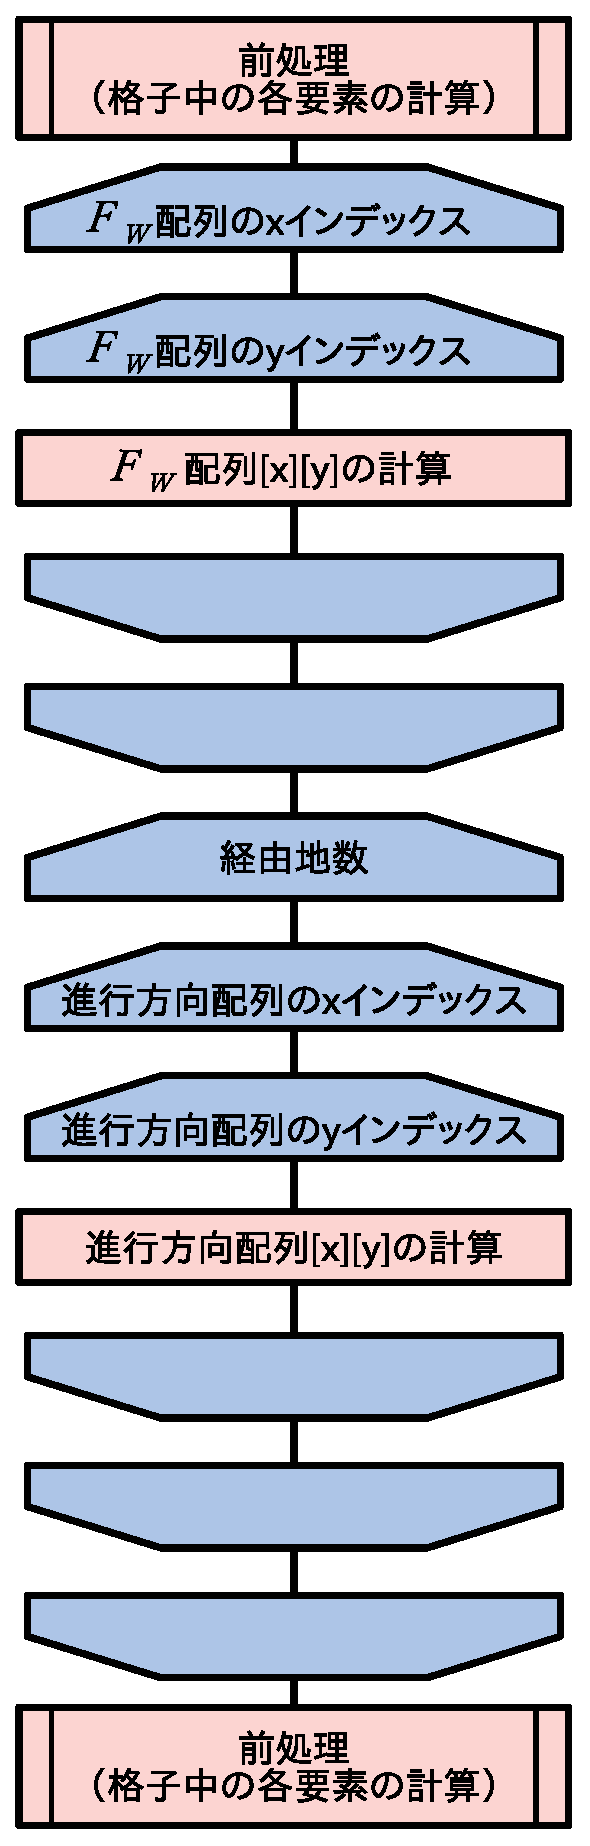
\includegraphics[width=4.5cm,clip]{figure/5_teian_flow2.eps}
  \caption{格子分割の前処理のフローチャート}
  \label{fig:5_teian_flow2}
 \end{center}
\end{figure}

\clearpage
\subsection{個別に進行方向を計算する格子の判定}
格子分割を用いた進行方向の計算回数削減手法は,精度の大幅な低下を防ぐために,
\figref{fig:ex2}のように目的地や障害物が含まれる格子とその周辺の格子に存在するエージェントを
個別に進行方向を計算するように設定する.
個別に進行方向する格子には,xとyの両方のベクトルに0が格納されているため,
解析中にエージェントが存在する格子に0ベクトルが格納されているか判定が必要となる.
\figref{fig:5_teian_flow2}に進行方向ベクトル$e$および障害物を避ける力$F_{iW}$の
解析中に個別計算するかどうかの判定のフローチャートを示す.
\figref{fig:5_teian_flow2}が示すフローチャートは,\figref{fig:5_teian_flow1}中の
解析中の運動方程式を用いた計算であり,エージェントの進行方向を求めるための計算である.
\figref{fig:5_teian_flow2}中の$F_{iW}$配列は障害物を避ける力$F_{iW}$を格納する配列,
進行方向配列は進行方向ベクトル$e$を格納する配列である.
\figref{fig:5_teian_flow2}に示すように,格子分割を用いた進行方向の計算回数削減手法は,
エージェントの座標から参照する配列の要素を求め,0ベクトルが格納されていない場合に
配列中の値を参照し,0ベクトルが格納されている場合に個別計算を行うことで解析中の
計算回数を削減する.

\figtb{提案手法の運動方程式計算のフローチャート}{}{9}{5_teian_flow3.eps}{5_teian_flow2}
%\figtb{シミュレーション中の$f_{iW}$計算のフローチャート}{}{8.5}{5_e_flow.eps}{5_e_flow}


\clearpage
\section{評価(工事中)}
SFMを用いた人流シミュレーションに対する
格子分割を用いた進行方向の計算回数削減手法の有効性を確認するために,
既存手法であるセル分割法と提案手法を用いて人流シミュレーション
評価環境は,\tabref{tb:result_env}に示すマシンである.
本評価では,\tabref{tb:result_para}に示すパラメータを用いて
SFMの運動方程式を計算する.
本評価では,避難時のシミュレーションを再現するために,
エージェント数よりも壁粒子が多い配置にエージェントを一方向に進むような解析を行う.
\figref{fig:haba2}と\figref{fig:haba5},\figref{fig:haba10},\figref{fig:haba20}に
本評価に用いる初期配置を示す.
図中の黒丸は壁粒子,紫色の丸はエージェント,青色の丸は目的地である.
図に示す配置のエージェントは40人,壁粒子は〇〇個,経由地は1個である.
図中のすべてのエージェントは,青色の丸が示す目的地に向かうように設定する.

\begin{table}[t]
  \begin{center}
    \caption{評価環境}
      \label{tb:result_env}
      \begin{tabular}{c|c}
      \hline \hline
      CPU              & Intel Xeon CPU E5-2667w v2 \\ \hline
      メモリ           & 32GB                       \\ \hline
      OS               & Linux 6.5.8               \\ \hline
      コンパイラ       & gcc 13.2.0                  \\ \hline
      最適化オプション & -O3                        \\ \hline
    \end{tabular}
  \end{center}
\end{table}

\begin{table}[t]
  \begin{center}
    \caption{測定条件}
    \label{tb:result_para}
    \begin{tabular}{c|c}
      \hline \hline
      $A_i$            & 2000N                              \\ \hline 
      $B_i$            & 0.08m                              \\ \hline 
      $k$              & $1.2 \times 10^5 kg s^{-2} $       \\ \hline 
      $\kappa$         & $2.4 \times 10^5 kg m^{-1} s^{-2}$ \\ \hline 
      $v_i^0$          & $1.4$m/s                           \\ \hline 
      $m_i$            & $80$kg                             \\ \hline 
      $\tau_i$         & 0.5                               \\ \hline 
      $r_i$            & $0.25$m                            \\ \hline 
      相互作用範囲     & $5$m                              \\ \hline 
    \end{tabular}
  \end{center}
\end{table}

\subsection{進行方向計算の計算回数}
%幅の測定のタイムステップは,3000ステップです.
本測定では,格子分割を用いた進行方向の計算回数削減手法の有効性を評価するために,
既存手法(セル分割法)と格子分割を用いた進行方向計算の回数削減手法の
計算回数を測定する.
測定する計算は,進行方向ベクトル$e$とエージェント間距離$d_{ij}$,壁を避ける力$f_{iW}$であり,
前処理の計算回数と解析中の計算回数の総和である.
\tabref{tb:haba2_times}から\tabref{tb:haba20_times}に配置ごとの各演算回数を示す.

\tabref{tb:haba2_times}から\tabref{tb:haba20_times}より,
提案手法は,どの通路幅においても進行方向ベクトル$e$の計算回数が削減できることがわかる.

\dfig{通路幅2mの初期配置}{20231023_haba2}{haba2}{通路幅5mの初期配置}{20231023_haba5}{haba5}

\dfig{通路幅10mの初期配置}{20231023_haba10}{haba10}{通路幅20mの初期配置}{20231023_haba20}{haba20}

\dfig{厚さ2倍}{haba2_2}{haba2_2}{厚さ3倍}{haba2_3}{haba2_3}

\begin{table}[t]
  \centering
  \caption{幅2mの計算回数[回]}
  \label{tb:haba2_times}
  \begin{tabular}{r|r|r|r}
  \hline \hline
          & 進行方向ベクトル$e$ & エージェント間距離$d_{ij}$ & 壁を避ける力$f_{iW}$ \\ \hline
    50.00 & 120000 & 4090023 & 25225464 \\ \hline
    25.00 & 120000 & 4090023 & 25225464 \\ \hline
    12.50 & 85821 & 4076346 & 25248928 \\ \hline
    6.25 & 46602 & 4092571 & 25229560 \\ \hline
    3.12 & 36236 & 4064182 & 25290728 \\ \hline
    1.56 & 21757 & 4076729 & 25279752 \\ \hline
    0.78 & 10797 & 4089809 & 25184712 \\ \hline
    0.39 & 2978 & 3836216 & 12672856 \\ \hline
    0.19 & 849 & 3738185 & 15438664 \\ \hline
    0.09 & 440 & 3909087 & 29316784 \\ \hline
    0.04 & 208 & 3972287 & 83614880 \\ \hline
    0.02 & 136 & 4067447 & 338197848 \\ \hline
    0.01 & 79 & 4097481 & 1314075632 \\ \hline
  \end{tabular}
\end{table}

\begin{table}[t]
  \centering
  \caption{幅5mの計算回数[回]}
  \label{tb:haba5_times}
  \begin{tabular}{r|r|r|r}
  \hline \hline
    & 進行方向ベクトル$e$ & エージェント間距離$d_{ij}$ & 壁を避ける力$f_{iW}$ \\ \hline
    50.00 & 120000 & 4688353 & 25456584 \\ \hline
    25.00 & 120000 & 4688353 & 25456584 \\ \hline
    12.50 & 88503 & 4681867 & 25472272 \\ \hline
    6.25 & 50471 & 4689221 & 25449696 \\ \hline
    3.12 & 40568 & 4685846 & 25473036 \\ \hline
    1.56 & 26145 & 4688548 & 25519296 \\ \hline
    0.78 & 12177 & 4690114 & 15310712 \\ \hline
    0.39 & 3329 & 4667880 & 11812128 \\ \hline
    0.19 & 999 & 4673550 & 15628648 \\ \hline
    0.09 & 171 & 4691341 & 27346592 \\ \hline
    0.04 & 633 & 4689957 & 92133096 \\ \hline
    0.02 & 56 & 4688792 & 306084120 \\ \hline
    0.01 & 71 & 4688649 & 1312357208 \\ \hline
  \end{tabular}
\end{table}


\begin{table}[t]
  \centering
  \caption{幅10mの計算回数[回]}
  \label{tb:haba10_times}
  \begin{tabular}{r|r|r|r}
  \hline \hline
          & 進行方向ベクトル$e$ & エージェント間距離$d_{ij}$ & 壁を避ける力$f_{iW}$ \\ \hline
    50.00 & 120000 & 4795258 & 21142956 \\ \hline
    25.00 & 120000 & 4795258 & 21142956 \\ \hline
    12.50 & 83748 & 4796443 & 20908708 \\ \hline
    6.25 & 41698 & 4749379 & 22060416 \\ \hline
    3.12 & 33785 & 4788528 & 21266744 \\ \hline
    1.56 & 22287 & 4795440 & 11418180 \\ \hline
    0.78 & 8512 & 4794687 & 6968740 \\ \hline
    0.39 & 2200 & 4795356 & 9522400 \\ \hline
    0.19 & 611 & 4794782 & 11900008 \\ \hline
    0.09 & 181 & 4794855 & 24206932 \\ \hline
    0.04 & 75 & 4795260 & 89404732 \\ \hline
    0.02 & 22 & 4794879 & 333616556 \\ \hline
    0.01 & 78 & 4793933 & 1310055356 \\ \hline
  \end{tabular}
\end{table}


\clearpage
\subsection{シミュレーションの実行時間の測定}

\subsection{シミュレーション精度の測定}

\subsection{実問題に対する提案手法の有効性}

\section{本章のまとめ(工事中)}
工事中.

%***** END ************************************************
